\documentclass[tikz, border=2pt]{standalone}
\usepackage{tikz}
\usepackage{pgfplots}
\usetikzlibrary{decorations.pathreplacing,calc}
\begin{document}
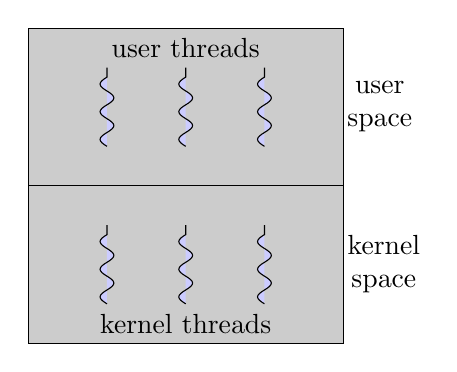
\begin{tikzpicture}
    \draw [fill=black!20] (0,2) rectangle (4,4);
    \draw [fill=black!20] (0,0) rectangle (4,2);
    \foreach \x in {1,...,3}
    {
        \draw[fill=blue!20, decorate,decoration={coil,aspect=0}] (\x,0.5) -- (\x,1.5);
        \draw[fill=blue!20, decorate,decoration={coil,aspect=0}] (\x,2.5) -- (\x,3.5);
    }
    \node [below] at (2,4) {user threads};
    \node [above] at (2,0) {kernel threads};
    \node [align=center, left] at (5,3) {user\\space};
    \node [align=center, left] at (5.1,1) {kernel\\space};
\end{tikzpicture}
\end{document}